% SPDX-FileCopyrightText: Copyright (c) 2023 Yegor Bugayenko
% SPDX-License-Identifier: MIT

\documentclass{article}
\usepackage[nominutes,template,scheme=dark]{ppt-slides}
\usepackage[static]{clicks}
\usepackage{multicol}
\usepackage[synonym=hs,colored,color=orange]{handstroke}
\usepackage{../../lecture-notes/notes}
\usepackage{svg}
\usepackage{tikz}
  \usetikzlibrary{shadows}

\graphicspath{{../../faces/}}

\definecolor{purewhite}{HTML}{FFFFFF}
\definecolor{myblack}{HTML}{000000}
\definecolor{myred}{HTML}{ED474A}
\definecolor{myblue}{HTML}{241CA6}

\newcommand\citch[1]{
  \plush{
  \begin{textblock}{10}[0.5,0.5](8,8)%
    \centering #1%
  \end{textblock}
  }}

\newcommand\pitch[6]{
  \lnPitch{
    \pptBanner{\bi{#1}{#2}}%
    \vspace*{2em}%
    {\large\enquote{\bi{#3}{#4}}}\par%
    \href{#5}{#6}}}

\newcommand\bi[2]{#1}

\RemoveFromHook{enddocument}[notes]

\begin{document}

\newcommand*{\thedate}{\bi{October 9th, 2026}{9 Октября 2026}}
\newcommand*{\thetitle}{\bi{What Are You, Human?}{Зачем ты мне, человек?}}
\newcommand*{\thesubtitle}{}
\newcommand*{\theauthor}{\bi{Yegor Bugayenko}{Егор Бугаенко}}

\pptLeft{%
  \begin{textblock}{3}(1,1)%
    \includesvg[height=3em]{logo.svg}
  \end{textblock}%
  \thedate
}
\pptRight{@yegor256}

\plush{
  \begin{textblock}{5}(9,0)%
    \tikz \node[minimum width=\paperwidth, minimum height=\paperheight, fill=purewhite, inner sep=0pt] {};
  \end{textblock}%
  \begin{textblock}{8}[1,1](15,15)%
    \raggedleft%
    
\includegraphics[width=.6\linewidth]{robot.jpg}
  \end{textblock}%
  \begin{textblock}{10}[0.5,0.5](6.5,7)
    \pptTitle{{\textcolor{black}{\thetitle}}}{}\par
    \textcolor{white}{\theauthor{} @ Zerocracy}\\
    \textcolor{white}{\thedate}
  \end{textblock}
  \begin{textblock}{10}[0.5,0.5](6.5,12)
    \includesvg[height=4em]{logo.svg}
  \end{textblock}
}
\newpage

\lnQuote
  {bernard-shaw}
  {The true joy in life is \hs{being used} for a mighty purpose.}
  {shaw1903man}

\lnQuote
  {alfred-adler}
  {A man makes himself useful to someone else [...] In this way he acquires a sense of his worth to society---the only possible means of mitigating the universal human feeling of \hs{inferiority}.}
  {adler1933social}

\lnQuote
  {robert-reich}
  {Symbolic-analytic services do not enter world commerce as standardized things. Traded instead are the \hs{manipulations of symbols}---data, words, oral and visual representations.}
  {reich1991work}

\citch{%
  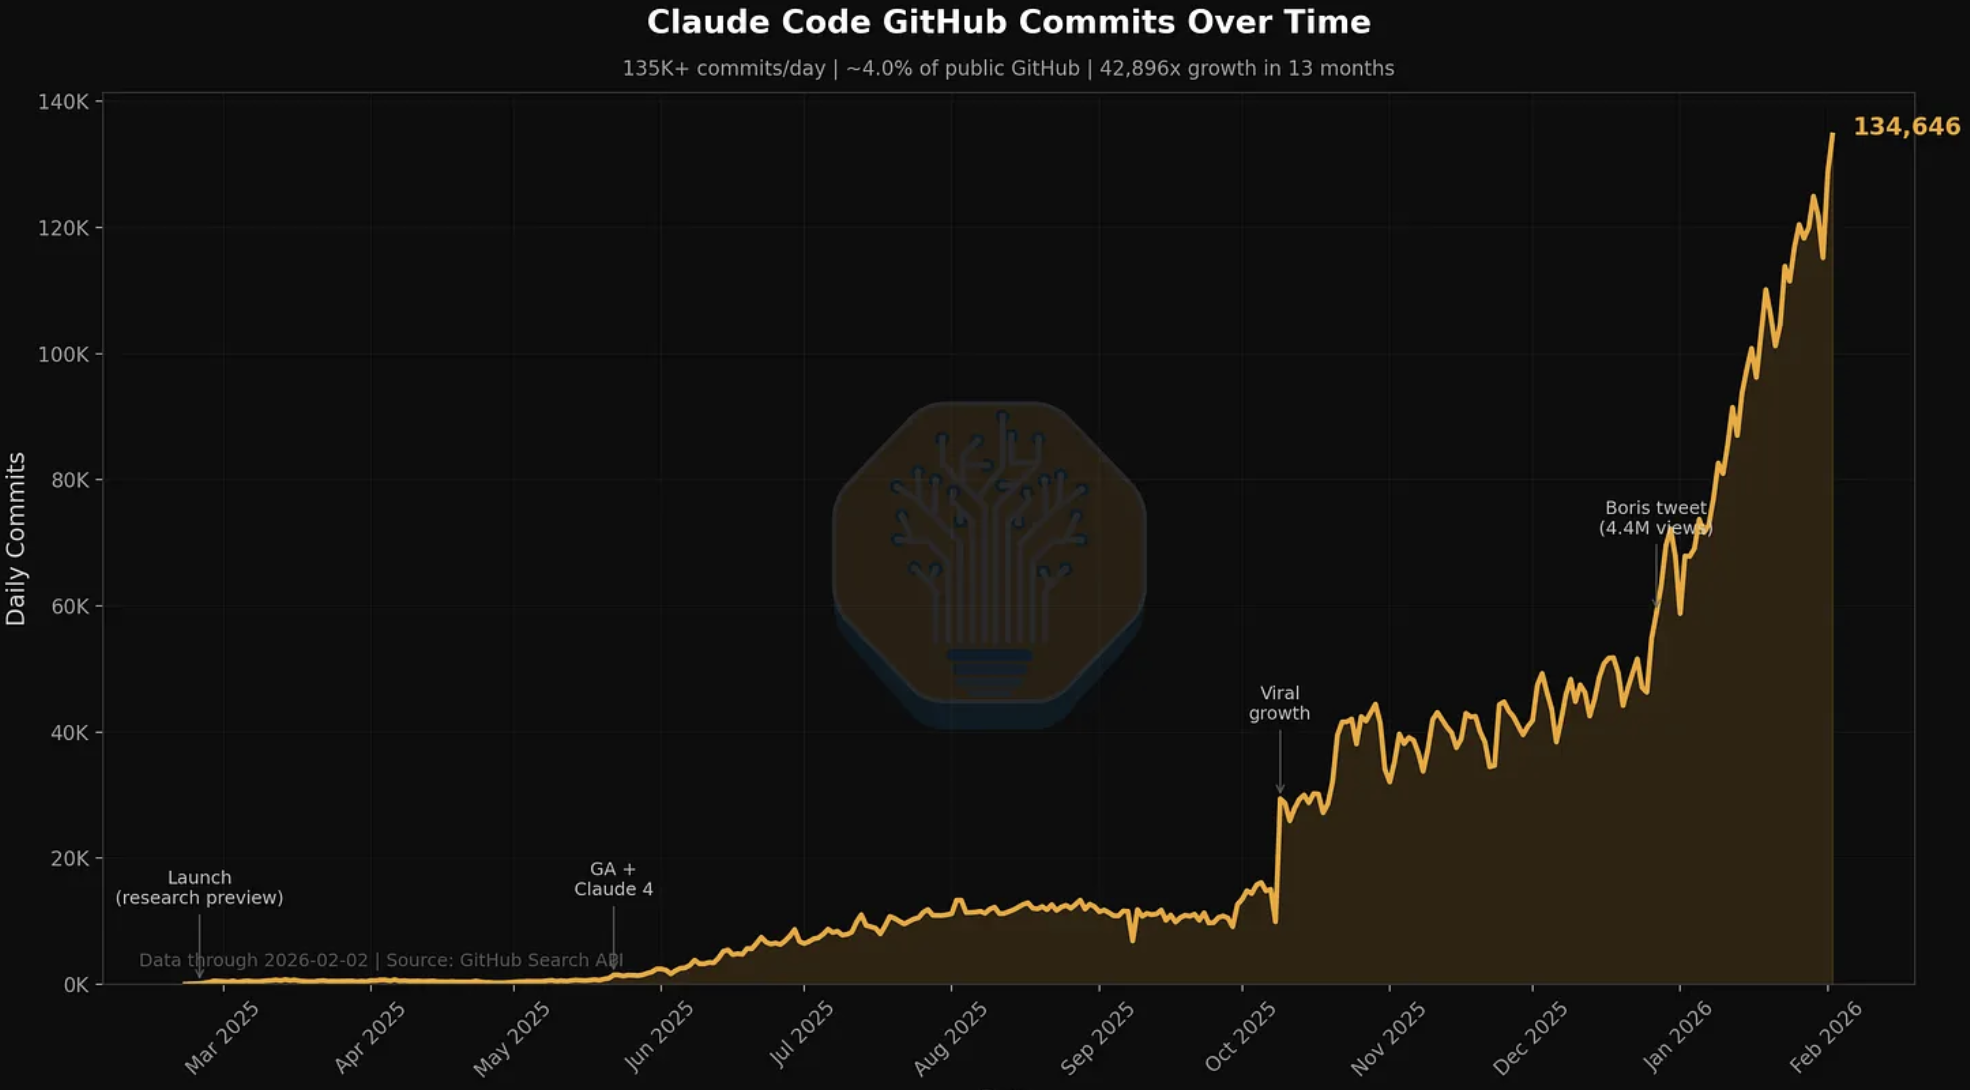
\includegraphics[width=.9\linewidth]{4-percent.png}
  \par
  In February 2026, SemiAnalysis \href{https://newsletter.semianalysis.com/p/claude-code-is-the-inflection-point}{showed} that
  \hs{4\%} of GitHub public commits are being authored by Claude Code.
  \par
  }

\citch{%
  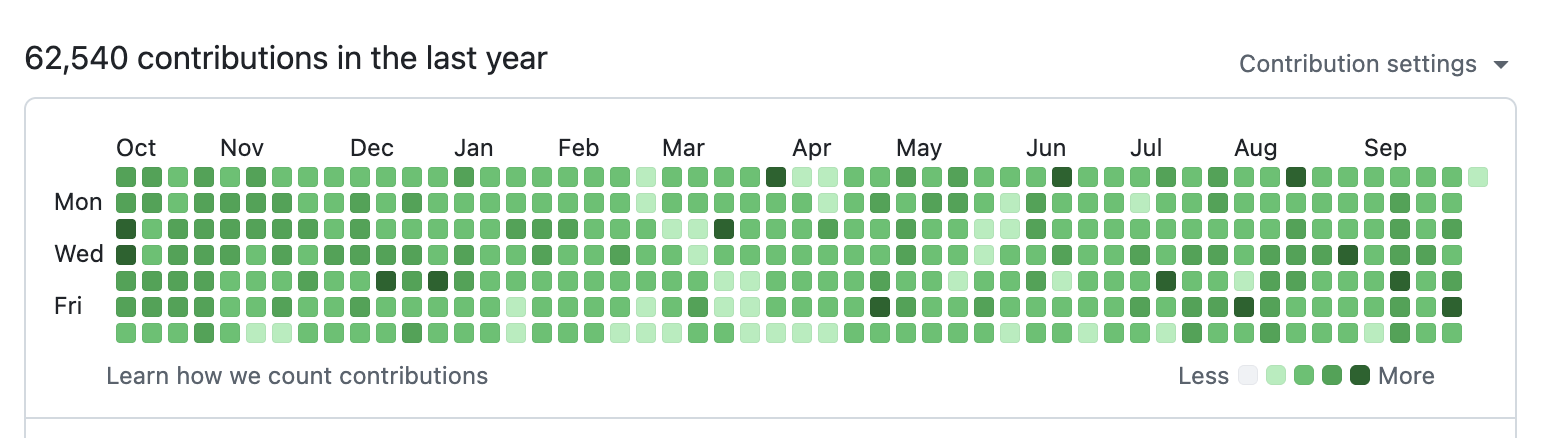
\includegraphics[width=.9\linewidth]{github.png}
  \par
  \href{https://github.com/yegor256}{@yegor256} (5.3K followers)
  \par
  I'm top-3 GitHub contributor in China: \href{https://committers.top/china}{committers.top}.
  \par
  \hs{100\%} commits made by Claude Code.
  }

\citch{%
  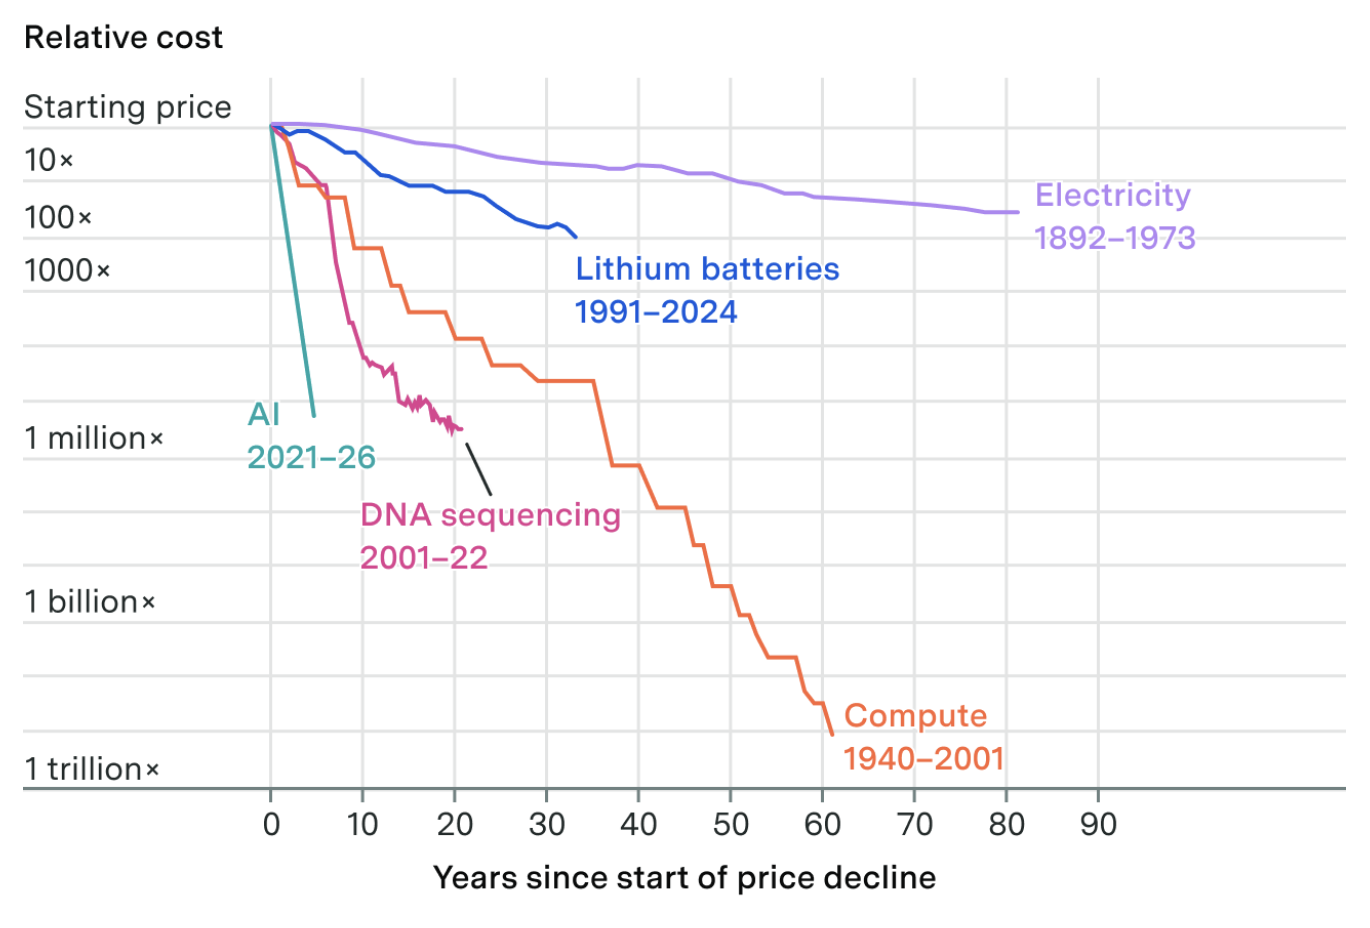
\includegraphics[width=.7\linewidth]{13-times.png}
  \par
  Every year LLMs are \href{https://epoch.ai/publications/the-plunging-price-of-thought}{getting}
  \hs{13 times} cheaper.
  \par
  }

\citch{%
  
\includegraphics[width=.6\linewidth]{server-room.jpg}
  \par
  Soon, humans will be \hs{prohibited} from touching the code.
  \par
  }

\lnQuote
  {yuval-noah-harari}
  {This \enquote{useless class} will not merely be unemployed --— it will be \hs{unemployable}.}
  {harari2017rise}

\lnQuote
  {hannah-arendt}
  {What we are confronted with is the prospect of a society of \hs{laborers without labor}, that is, without the only activity left to them. Surely, nothing could be worse.}
  {arendt1958human}

\citch{%
  
\includegraphics[width=.8\linewidth]{huang.jpg}
  \par
  In May 2026 Jensen Huang \href{https://www.youtube.com/live/FZh_0uRgrg4}{told}
  a graduating class at Carnegie Mellon:
  "Electricians, plumbers, iron workers, technicians, builders---this is your time."
  \par
  }

\citch{%
  
\includegraphics[width=.8\linewidth]{genie.jpg}
  \par
  A mortal human is giving an immortal genie the \hs{meaning of life}.
  \par
  }

\citch{%
  \qrcode[height=12em]{https://t.me/yegor256news}
  \par
  \href{https://t.me/yegor256news}{@yegor256news}
  \par
  }

\end{document}
